\documentclass[11pt]{report}
\usepackage[utf8]{inputenc}
\usepackage[T1]{fontenc}
 \usepackage{listings}
\usepackage{amsmath}

\usepackage{fancyhdr}
\usepackage{graphicx}
\usepackage{color}
\pagestyle{fancy}


 \lhead{Geoffrey PERRIN - Océane DUBOIS}
 \rhead{}
 \rfoot{}




\definecolor{codegreen}{rgb}{0,0.6,0}
\definecolor{codegray}{rgb}{0.5,0.5,0.5}
\definecolor{codepurple}{rgb}{0.58,0,0.82}
\definecolor{backcolour}{rgb}{0.95,0.95,0.92}

\lstdefinestyle{mystyle}{
    backgroundcolor=\color{backcolour},
    commentstyle=\color{codegreen},
    keywordstyle=\color{magenta},
    numberstyle=\tiny\color{codegray},
    stringstyle=\color{codepurple},
    basicstyle=\footnotesize,
    breakatwhitespace=false,
    commentstyle=\color{codegreen},
    breaklines=true,
    captionpos=b,
    keepspaces=true,
    numbers=left,
    numbersep=5pt,
    showspaces=false,
    showstringspaces=false,
    showtabs=false,
    tabsize=2,
     morekeywords={mov, push, xor, extern, div, mov, inc, cmp, jne, call, pop, ret,endp, proc, end, dec, add, jb, dd, db, jge,  not, lea, main, public, movzx, movd, psllq,imul, movq, pxor, sub, paddw, punpcklbw, pmaddwd, phaddd, shr, psrld, ja},
   extendedchars=true,
    sensitive=false,
   morecomment=[l];,
    literate= {á}{{\'a}}1 {é}{{\'e}}1 {í}{{\'i}}1 {ó}{{\'o}}1 {ú}{{\'u}}1 {Á}{{\'A}}1 {É}{{\'E}}1 {Í}{{\'I}}1 {Ó}{{\'O}}1 {Ú}{{\'U}}1 {à}{{\`a}}1 {è}{{\`e}}1 {ì}{{\`i}}1 {ò}{{\`o}}1 {ù}{{\`u}}1 {À}{{\`A}}1 {È}{{\'E}}1 {Ì}{{\`I}}1 {Ò}{{\`O}}1 {Ù}{{\`U}}1 {ä}{{\"a}}1 {ë}{{\"e}}1 {ï}{{\"i}}1 {ö}{{\"o}}1 {ü}{{\"u}}1 {Ä}{{\"A}}1 {Ë}{{\"E}}1 {Ï}{{\"I}}1 {Ö}{{\"O}}1 {Ü}{{\"U}}1 {â}{{\^a}}1 {ê}{{\^e}}1 {î}{{\^i}}1 {ô}{{\^o}}1 {û}{{\^u}}1 {Â}{{\^A}}1 {Ê}{{\^E}}1 {Î}{{\^I}}1 {Ô}{{\^O}}1 {Û}{{\^U}}1,
  }

\lstset{style=mystyle}

%Gummi|065|=)
\title{\textbf{TP08 - Traitement d'image - Troisième Partie }
\author{Geoffrey PERRIN \\ Océane DUBOIS\\}
\date{}}

\begin{document}

\maketitle

\newpage

Le but de ce TP est d'utiliser l'extension SSE pour aller plus vite lors des calculs et obtenir un programme plus condensé.
On commence par traiter les pixels 2 par 2, puis on traitera les pixel 4 par 4.

On commence donc par charger les 2 derniers pixels de l'image dans un registre, puis à l'aide de l'instruction "unpack" on sépare chaque composante RVB par mot de 0000. Ensuite on charge les coefficients multiplicateurs dans un registre, puis on les place en double dans un registre xmm2.
On unpack également xmm2, ainsi on se retrouve avec les coefficients multiplicateurs alignés avec chaque valeur RVB correspondante.

Grâce à l'instruction pmaddd, on multiplie les coefficients avec les valeur RVB puis on les additionne 2 à 2.

Afin d'avoir les 3 résultats additionés ensemble, on complète l'instruction par un phadd. On se retrouve avec 2 fois le résultat du pixel 1 et 2 fois le résultat du pixel 2 enregistré en xmm0.

On récupère d'abord dans eax le résultat du pixel 1, qu'on divise par 256 (car les coefficients sont à virgule fixe). Puis on place ce résultat dans le pixel de destination.
On réalise la même opération pour le pixel 2.

On réalise ces opération tant qu'il y a des pixels à traiter.


\begin{lstlisting}
; IMAGE_SIMD.ASM
;
; MI01 - TP Assembleur 2 à 5
;
; R?alise le traitement d'une image 32 bits.

.686
.XMM
.MODEL FLAT, C

.DATA

.CODE

; **********************************************************************
; Sous-programme _process_image_simd
;
; R?alise le traitement d'une image 32 bits avec des instructions SIMD.
;
; Entrées sur la pile : Largeur de l'image (entier 32 bits)
;           Hauteur de l'image (entier 32 bits)
;           Pointeur sur l'image source (d?pl. 32 bits)
;           Pointeur sur l'image tampon 1 (d?pl. 32 bits)
;           Pointeur sur l'image tampon 2 (d?pl. 32 bits)
;           Pointeur sur l'image finale (d?pl. 32 bits)
; **********************************************************************
PUBLIC      process_image_simd
process_image_simd   PROC NEAR       ; Point d'entrée du sous programme

        push    ebp
        mov     ebp, esp

        push    ebx
        push    esi
        push    edi

        mov     ecx, [ebp + 8]
        imul    ecx, [ebp + 12]
		sub		ecx,2

        mov     esi, [ebp + 16]
        mov     edi, [ebp + 20]

	;chargement des coeff

	mov eax, 4C961Dh
	movd xmm2, eax
	psllq xmm2, 32
	movd xmm1, eax
	paddw xmm1,xmm2
	pxor xmm3, xmm3
	punpcklbw  xmm1, xmm3


boucle:
  ;on récupère deux pixels de l'image source à traiter
  movq xmm0, qword ptr[esi+ecx*4]
	punpcklbw  xmm0, xmm3
	pmaddwd xmm0, xmm1
	phaddd xmm0,xmm3

  ;premier pixel
	movd eax, xmm0 ;on récupère le premier coefficient
	shr eax, 8 ;on divise par 256
	mov [edi+ecx*4], eax

	psrlq xmm0, 32

  ;deuxieme pixel
	movd eax, xmm0
	shr  eax, 8
	mov [edi+ecx*4+4], eax

	sub ecx, 2
  ja     boucle

fin:
        pop     edi
        pop     esi
        pop     ebx

        pop     ebp

        ret                         ; Retour à la fonction MainWndProc

process_image_simd   ENDP
END


\end{lstlisting}


TEMPS !!!!!

\newpage
Pout adapter la boucle qui itère sur les pixels de l’image pour prendre en compte quatre pixels par itération
au lieu de deux il suffit de soustraire 4 à ecx a la fin de chaque itération.

L'instruction movdqa xmm0, oword ptr[esi+ecx*4] permet de récupérer 128 bits en mémoire soit 4 pixels de 32 bits avec 4 composantes de 8bits.

Pour faire le calcul, on peut exploiter l’instruction pmaddubsw. Il s’agit d’une multiplicationaddition
qui considère deux vecteurs d’octets (l’un signé et l’autre non signé) et
produit ses résultats sous forme d’un vecteur de mots signés de 16 bits. Le vecteur d'octet si il est signé ne peut comporter des valeurs uniquement entre -128 et 127.
Dans notre cas le niveaux de gris I peut varier de 0 255 (somme des coeffs = 1).
Si on suppose que les coefficients sont pair on peut les diviser par deux pour que la somme des coeffs = 0.5
Ainsi le niveau de gris I d'un pixel varira entre 0 et 255*0.5 soit 127
Il faut donc arrondir nos coefficient au nombre pair superieur si ils sont impair pui diviser par deux.
Voici le snouveaux coefficients 264b0Eh.

Construire un second vecteur d’octets qui contient les constantes associées à chaque
composante de chaque pixel, toujours au moyen d’instructions de type « unpack »:
\\
\\mov eax, 264b0Eh
-> Ici on met les coefficients dans les 32 bits de poid faible de xmm2
\\psllq xmm2, 32
-> On décale de 32 bits a gauche
\\movd xmm1, eax
-> On met les coefficients dans les 32 bits de poid faible de xmm1
\\paddw xmm1,xmm2
-> On additionne les vecteurs de 16 bits des registres xmm1 et xmm2 entre eux afin d'avoir les coefficients sur les 64 bits de poid faible de xmm1
\\punpckldq xmm1,xmm1
-> On effectue unpack pour propager les coefficients sur les 128 bits de xmm1

\begin{figure}[h]
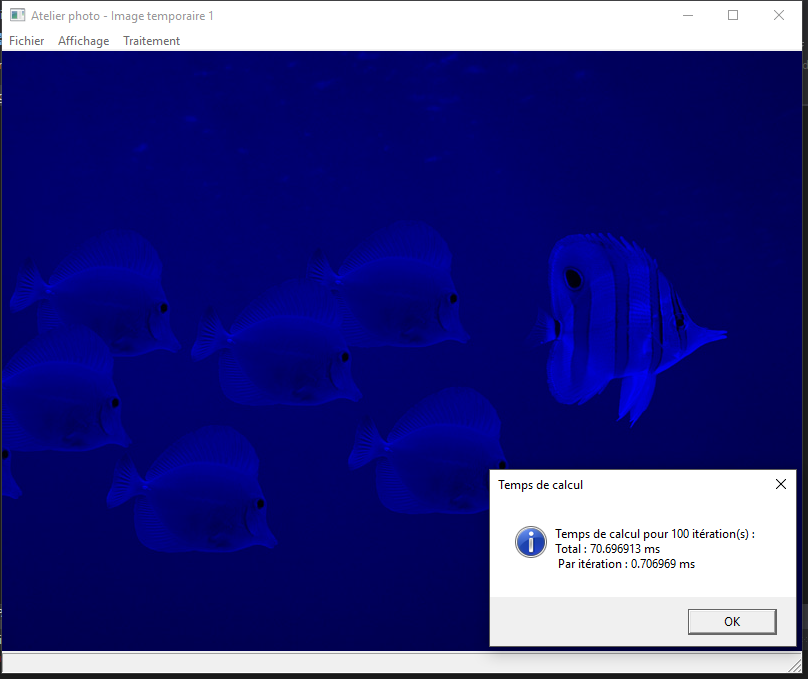
\includegraphics[width=13cm]{Capture1.png}
\caption{Mise en place des coefficients}
\end{figure}


\\Faire le calcul d’intensité à partir de ces deux vecteurs, en prenant garde aux décalages
nécessaires de la virgule: voir le code commenté et le schema ci-dessous:
\begin{figure}[h]
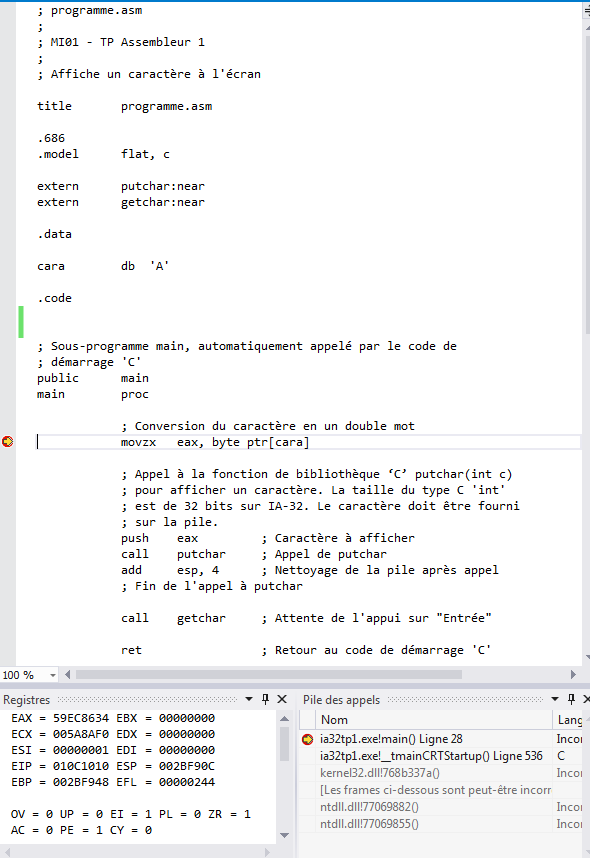
\includegraphics[width=13cm]{Capture2.png}
\caption{Calcul d'intensité pour 4 pixels}
\end{figure}

Stocker le résultat de ces calculs dans l’image résultante:
movdqa [edi+ecx*4], xmm0
On copie simplement le contenu de xmm0 en mémoire grace a cette instruction.


\newpage
Voici le code :

\begin{lstlisting}

; IMAGE_SIMD.ASM
;
; MI01 - TP Assembleur 2 à 5
;
; R?alise le traitement d'une image 32 bits.

.686
.XMM
.MODEL FLAT, C

.DATA

.CODE

; **********************************************************************
; Sous-programme _process_image_simd
;
; R?alise le traitement d'une image 32 bits avec des instructions SIMD.
;
; Entrées sur la pile : Largeur de l'image (entier 32 bits)
;           Hauteur de l'image (entier 32 bits)
;           Pointeur sur l'image source (d?pl. 32 bits)
;           Pointeur sur l'image tampon 1 (d?pl. 32 bits)
;           Pointeur sur l'image tampon 2 (d?pl. 32 bits)
;           Pointeur sur l'image finale (d?pl. 32 bits)
; **********************************************************************
PUBLIC      process_image_simd
process_image_simd   PROC NEAR       ; Point d'entrée du sous programme

  push    ebp
  mov     ebp, esp

  push    ebx
  push    esi
  push    edi

  mov     ecx, [ebp + 8]
  imul    ecx, [ebp + 12]

  mov     esi, [ebp + 16]
  mov     edi, [ebp + 20]
  sub      ecx,4

  ;mise en place des coeffs
  mov eax, 264b0Eh
  movd xmm2, eax
  psllq xmm2, 32
  movd xmm1, eax
  paddw xmm1,xmm2
  punpckldq xmm1,xmm1

boucle:

  ;on récupére les 4 pixel de l'image source à traiter
  movdqa xmm0, oword ptr[esi+ecx*4]
  ;on fait le calcul avec les coefficients de xmm1
  pmaddubsw xmm0,xmm1
  ;on ajoute la somme des deux premire composante de chaque pixels a la 3eme
  phaddw xmm0, xmm3
  ;on divise par 128 car les coeffs ont été divisé par 2
  psrlw xmm0,7
  ;on met le resultat du calcul dans la composante bleu
  punpcklwd xmm0,xmm3
  movdqa [edi+ecx*4], xmm0

sub	ecx,4
ja     boucle

fin:
pop     edi
pop     esi
pop     ebx

pop     ebp

ret

process_image_simd   ENDP
END

\end{lstlisting}

\newpage
Test de performance:

\begin{figure}[h]
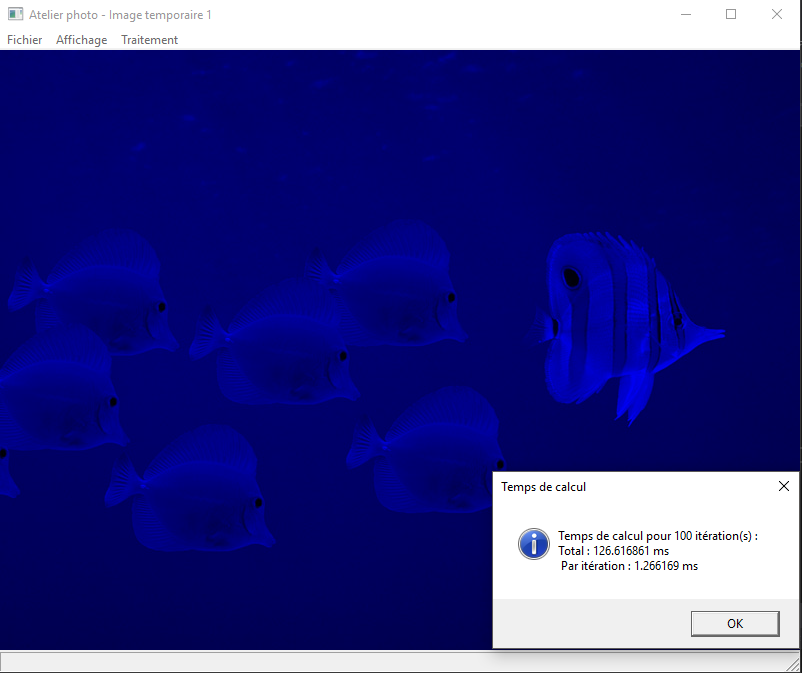
\includegraphics[width=13cm]{CaptureC.png}
\caption{Temps d'éxecution avec l'algorithme C}
\end{figure}

\begin{figure}[h]
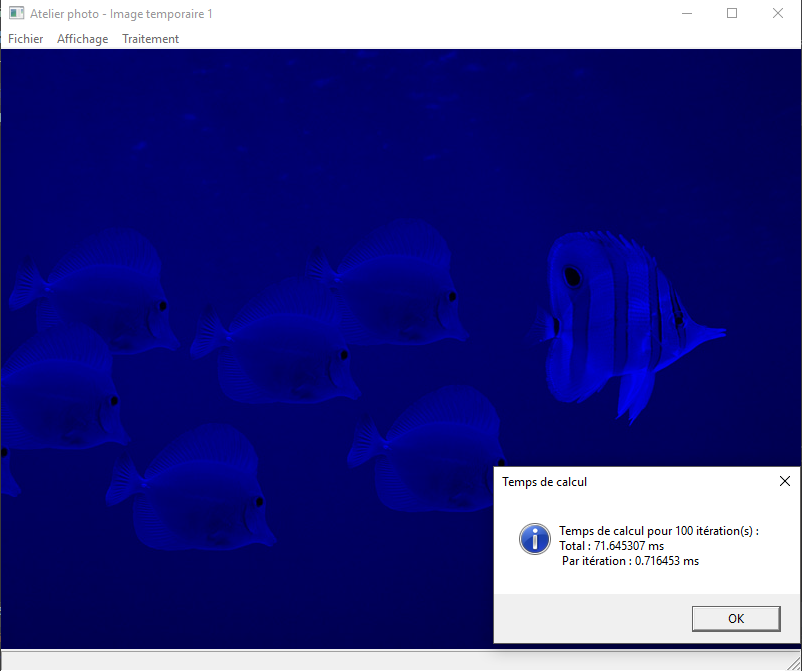
\includegraphics[width=13cm]{CaptureASM.png}
\caption{Temps d'éxecution avec l'algorithme ASM}
\end{figure}

\begin{figure}[h]
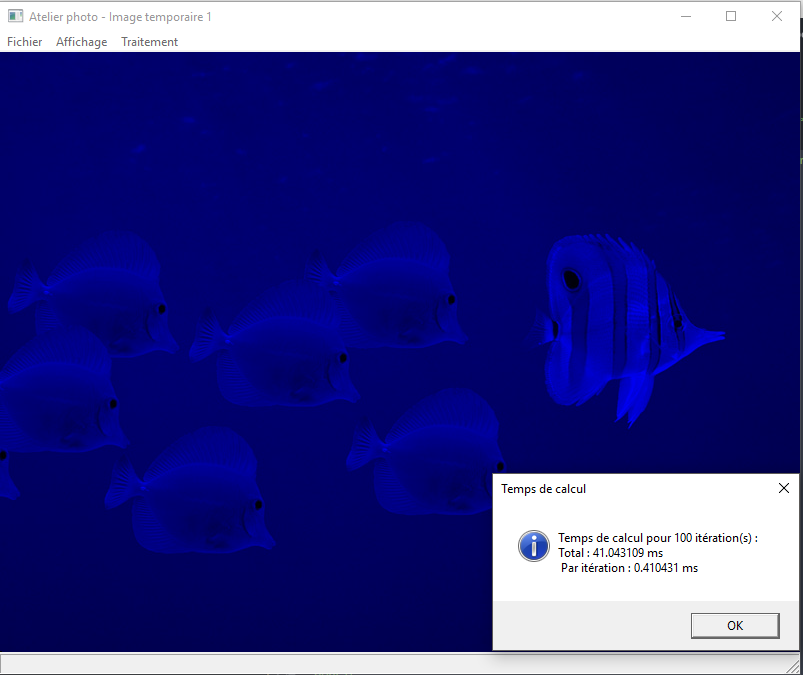
\includegraphics[width=13cm]{CaptureSimd2.png}
\caption{Temps d'éxecution avec l'algorithme SIMD avec 2 pixels}
\end{figure}

\begin{figure}[h]
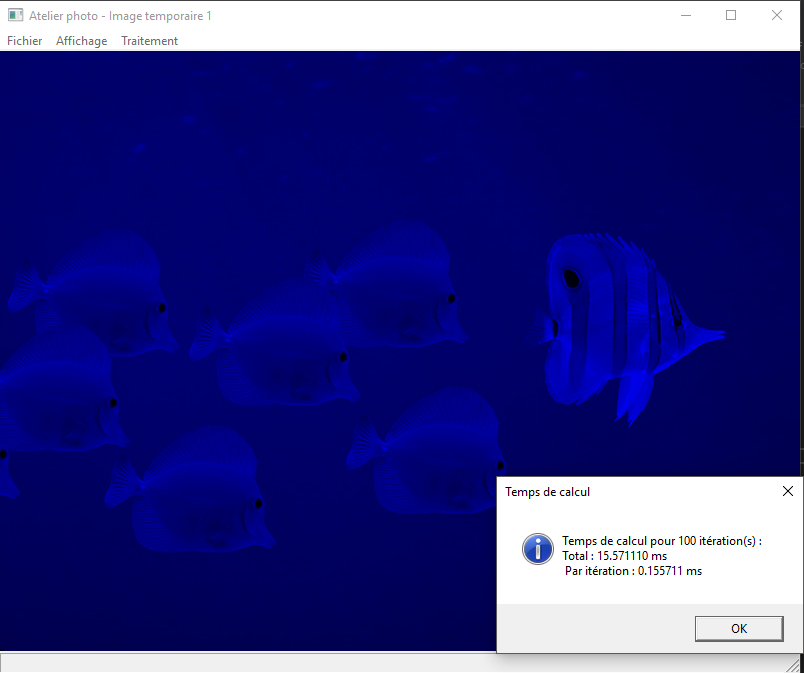
\includegraphics[width=13cm]{CaptureSimd4.png}
\caption{Temps d'éxecution avec l'algorithme SIMD avec 4 pixels}
\end{figure}

\\Le temps d'excution moyen par itération en C et de 1.2ms
\\En assembleur on divise par 1.7 ce temps avec 0.7ms de moyenne.
\\En SIMD avec un traitement de deux pixels on divise le temps par 3 par rapport au c avec 0.4ms de moyenne
\\Enfin en SIMD avec un traitement de quatre pixels on divise le temps par 8 par rapport au c avec 0.15ms de moyenne
Les gains de temps sont donc significatif à chaque fois. Grace au jeux d'instruction SIMD on peut optimiser avec un facteur de 8 un algorithme C


\end{document}
